
%%%
% Any line that begins with a percent symbol is a comment. To compile
% this document and view the output:
%
% Run Latex
% Run Bibtex
% Then run Latex twice.
%
% This should produce the output PDF file named main.pdf
%%%

% This defines the style to use for this document.
% Do not modify.
\documentclass[letterpaper]{article}

% The following are akin to "import" statements in Python or Java -
% these import useful commands into the document for you to use.  You
% don't have to modify any of these lines. The AAAI package formats
% this document in the style of submissions to the American
% Association for Artificial Intelligence conference, one of the top
% AI conferences in the world. You will find that many academic
% publications in AI use this format.
\usepackage{aaai} 
\usepackage{times} 
\usepackage{helvet} 
\usepackage{courier} 
\setlength{\pdfpagewidth}{8.5in} 
\setlength{\pdfpageheight}{11in} 
\usepackage{amsmath}
\usepackage{amsthm}
\usepackage{graphicx}
\usepackage{graphics}
\usepackage{moreverb}
\usepackage{subfigure}
\usepackage{epsfig}
\usepackage{txfonts}
\usepackage{palatino}
\usepackage{algpseudocode}
\usepackage{multirow, multicol}
\usepackage{url}
\usepackage{tablefootnote}
\usepackage{color}

\setcounter{secnumdepth}{1}
\nocopyright

% Fill in your paper title, names and emails below
% The "\\" is used to break lines. The \url command
% is useful for typesetting URLs and email addresses (it uses the
% Courier font).
\title{Implementing an Ant Swarm Intelligence-Based Approach to Balancing Communication Network Loads}
 \author{Ben Wiley \and Tommy Rhodes\\
 \url{{bewiley, torhodes}@davidson.edu}\\
 Davidson College\\
 Davidson, NC 28035\\
 U.S.A.}

% This is the "true" start of the document. All the text in your
% write-up should be placed within the \begin{document} and
% \end{document} decorators.
\begin{document}

\maketitle % formats the title nicely, do not modify

% While at this point you could just begin your write-up, often, it's
% useful to write each section of your write-up in a separate tex
% file (not unlike the modular decomposition you do for code you
% write). These \input commands insert the contents of the
% specified tex files in the order specified. Every write-up you
% submit must contain the following sections, in the shown order. Open
% each of the indicated tex files to understand what goes in each
% section, as well as for more TeX tips.

% Place the contents of your abstract between the
% \begin{abstract} and \end{abstract} decorators.

\begin{abstract}

The purpose of this project is to implement a swarm intelligence algorithm in order to solve load balancing in communications networks. We aim to reproduce the experiments of Schoonderwoerd et al., and compare their decentralized call routing algorithm’s performance with routing using a shortest path (breadth-first search) algorithm and a minimum-weight algorithm (Dijkstra’s Algorithm). The decentralized algorithm mimics the swarm behavior of an ant colony, and uses roaming, ant-like agents which drop probability “pheromones” on nodes in order to influence the travel behavior of fellow ants and to regulate the paths of calls made across the network. Each algorithm is evaluated on the basis of the number of calls dropped. Ignoring time complexity, Dijkstra performed best, followed by the ant-based algorithm and then breadth-first search.

% The \textbf{} command makes the specified text bold. The \emph{} or
% \textit{} command are used to italicize text. In general, text is never
% underlined.

% DON'T FORGET TO MATCH EACH OPEN BRACE WITH A CLOSING BRACE!
\end{abstract}



% The \section{} command formats and sets the title of this
% section. We'll deal with labels later.
\section{Introduction}
\label{sec:intro}

When researching for this project, we were interested in finding a context in which using swarm intelligence algorithms was a good option, and not just an algorithm that could be adapted in order to solve the given problem. In doing so, we came across the paper by Schoonderwoerd et al. and became interested in the ant-based approach to balance communications networks.\\

Because usage of telecommunications networks is increasing, this problem is very important. Managing load by efficiently and effectively distributing load across a network, especially with the ability to route around congested nodes of the network, is crucial in order to keep the network performing as it should. \\

\section{Background}
\label{sec:background}

With increasing traffic on telecommunications networks, effectively balancing the load across all nodes of the network is crucial to the network performing well. In other words, while shortest path algorithms may quickly find the optimal short-distance route between nodes in a call, an improved algorithm will bypass high congestion areas in order to make calls more efficient and avoid dropping calls on the network. In order to effectively balance loads, we look to the previous research done by Ruud Schoonderwoerd, Owen Holland, Janet Bruten, and Leon Rothkrantz on simulating pheromone trails of ants. As real-life ants follow paths, they drop pheromones to influence the behavior of other ants and improve the overall colony’s sense of navigation. The strength of the pheromones decreases over time, so ants that find paths that take less time have a larger influence on the paths taken by future ants. \\

\begin{figure}[htb]

  \centering
  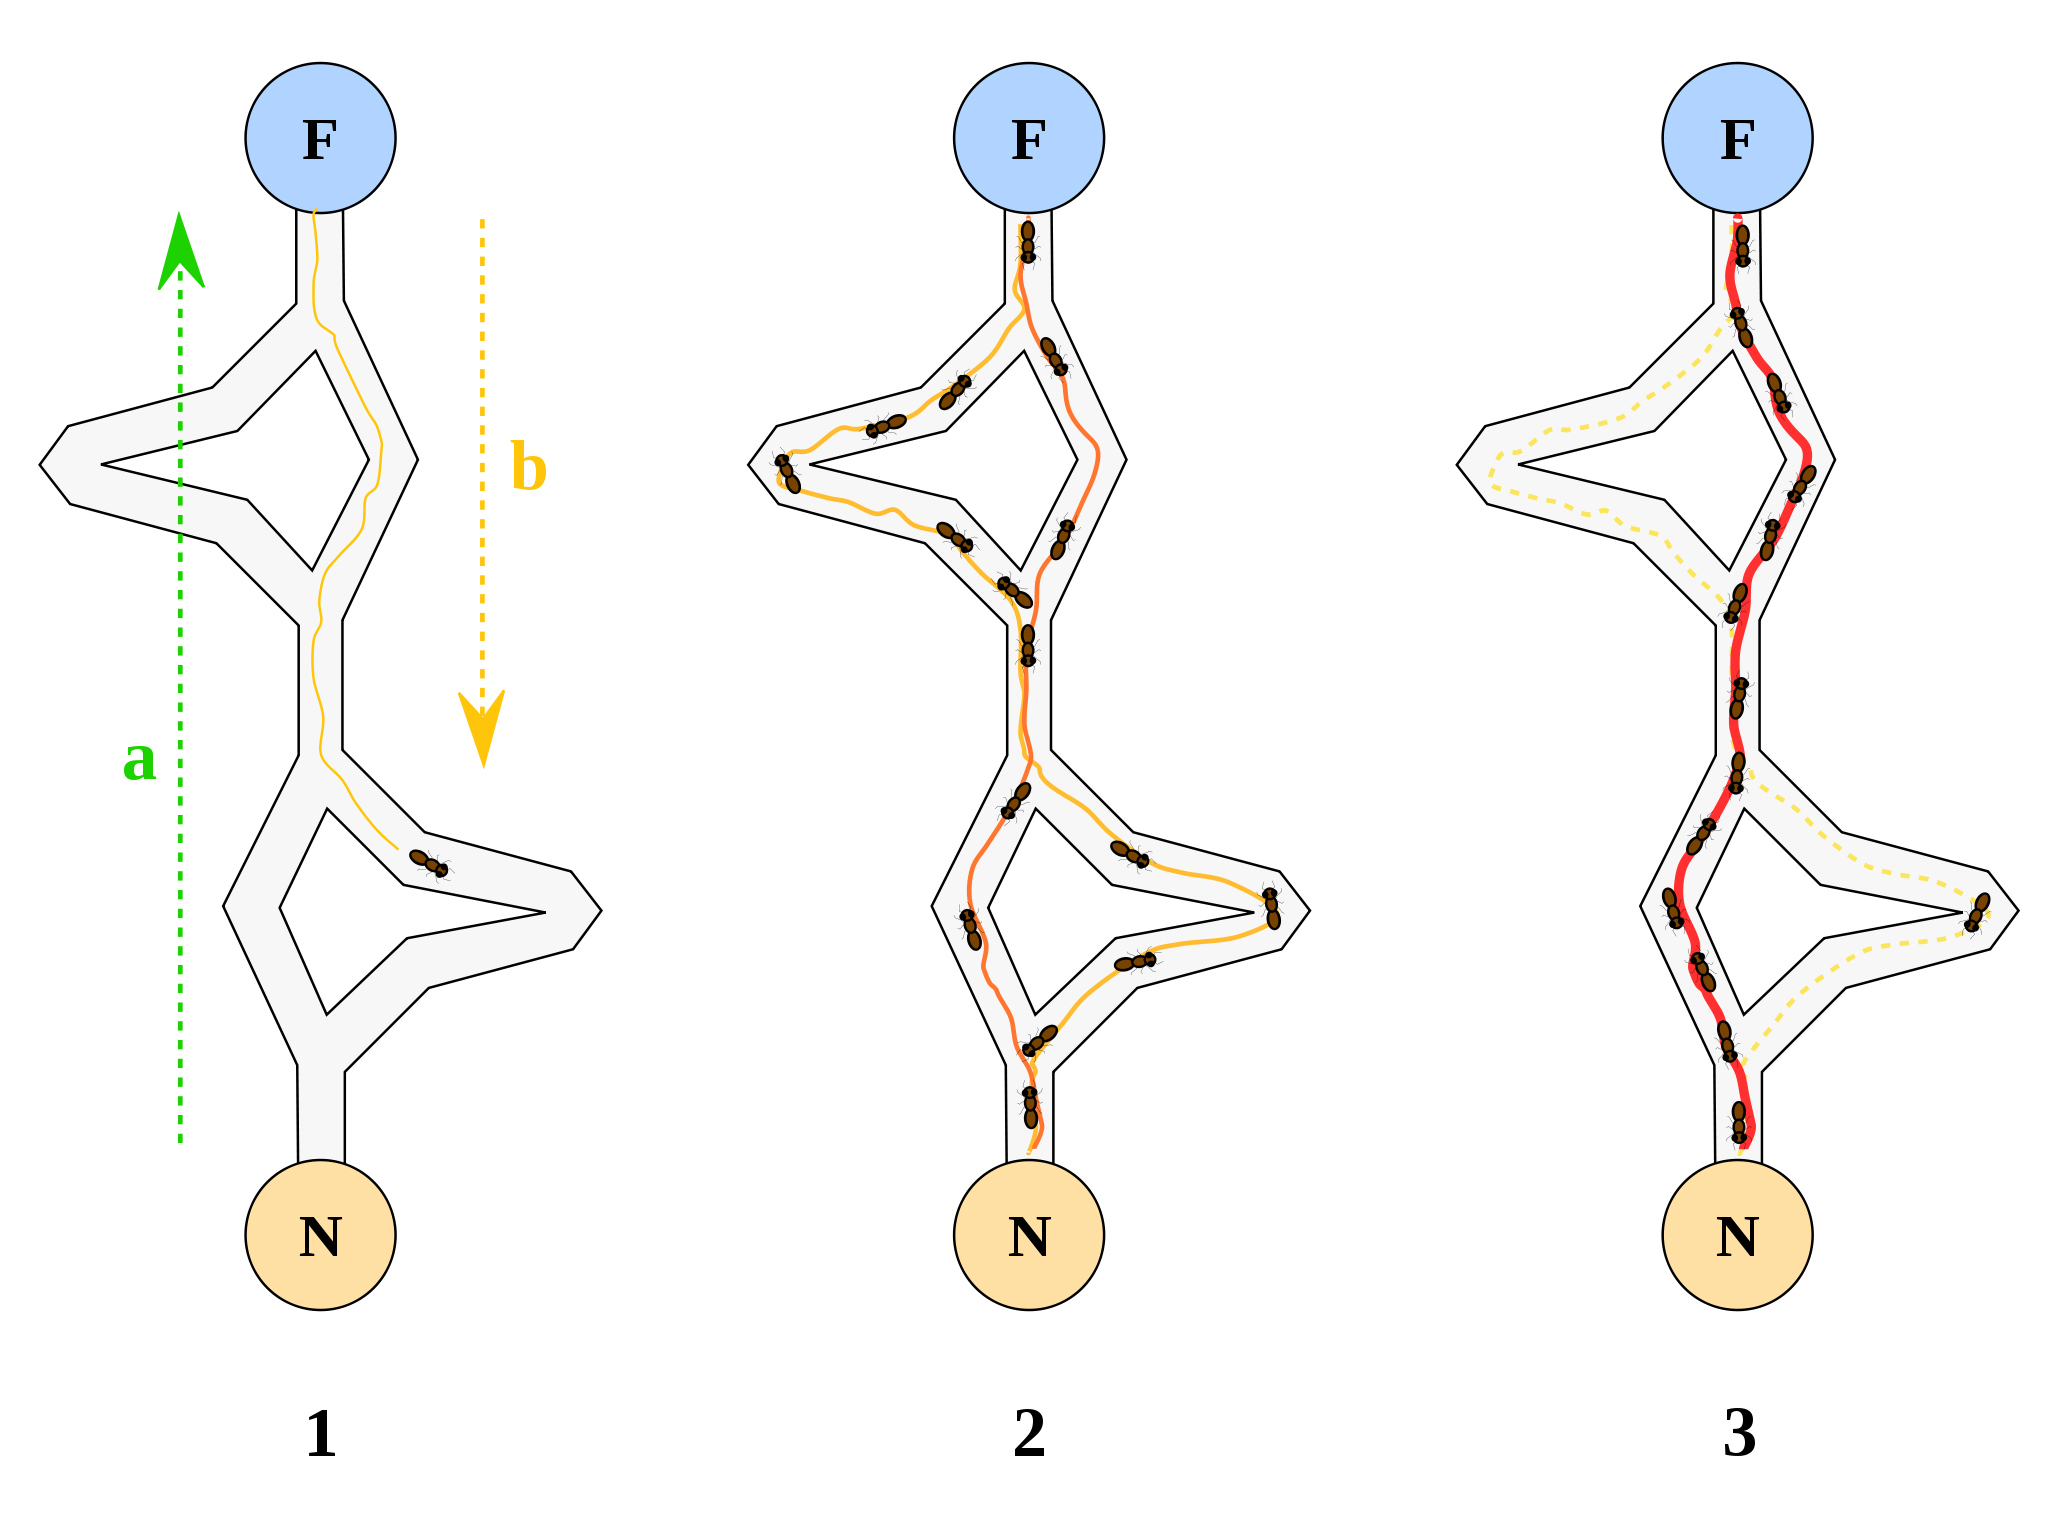
\includegraphics[width=0.47\textwidth]{figs/ants_nature.jpg}
  \caption{An example of ant colony routing over time. (Wikimedia Commons)}
  \label{fig:tex}

\end{figure}

Our algorithm adopts this approach using artificial ant-like agents to regulate local call routing. Ants become delayed on congested nodes, and have decaying influence on routing probabilities as a function of time spent on the network. The theory is that as an ant travels along a path, if the path is congested, the ant's pheromones will be weaker, so ants (and network calls) traveling in the future will be less likely to take that path.

\section{The Algorithm}
\label{sec:expts}

\subsection{Ants}
The algorithm works by employing ant-based mobile agents to traverse the network and attempt to find the least weight path across the network. It does so by mimicking the pheromone trails of ants. In the algorithm, an ant is deployed from each node once per time step. The ant chooses its destination in the network randomly, and then follows a path to that node by following the probabilities stored in each node. The tables include a row for each possible destination node and a column for each neighbor node. As an ant travels, it looks up the row of its destination node and chooses its next node based on the probabilities for each neighbor. When it visits a node, it also updates the probability table by changing the node the ant has just come from according to: $$p = \frac{p_{old} + \Delta p}{1 + \Delta p}$$ and decreases the rest of the probabilities according to: $$p = \frac{p_{old}}{1 + \Delta p}$$ where $\Delta p$ is a function of the age of the ant: $$\Delta p = \frac{0.08}{age} + 0.05$$ In order to simulate traffic on the network, ants are delayed in getting to nodes based on a function of the spare capaticy $s$ of the node: $$delay = 80e^{-0.075s}$$ When an ant is traveling between nodes, the age of the ant is determined by the delay function. This means that more congested nodes take longer for ants to get to, reducing their effect on the probability table.

\subsection{Call Routing}
Calls are routed between nodes based on the probability tables as well. Much like the ants, calls look at the row in the probability table that corresponds to the destination node. The call then chooses the largest probabillity in the neighbor nodes and chooses that neighbor as its next node. If at any point a call attempts to be routed through a node that has no spare capacity, the call is dropped.

\subsection{Parameters}
There are several parameters which we used in our experiment worth noting:\\

-The average length of a call is 170 time steps. We used a Gaussian distribution with a mean of 170 and a standard deviation of 20 to model this.\\

-On average, one call is made every time step.\\

-One ant is released from each node at every time step.\\

-The maximum load on each node is 40 calls.\\

-Calls are made based on a uniform distribution of source and destination nodes.\\

-The graph used to model the network is the British Telecommunications core network circa 1996.\\

\begin{figure}[htb]

  \centering
  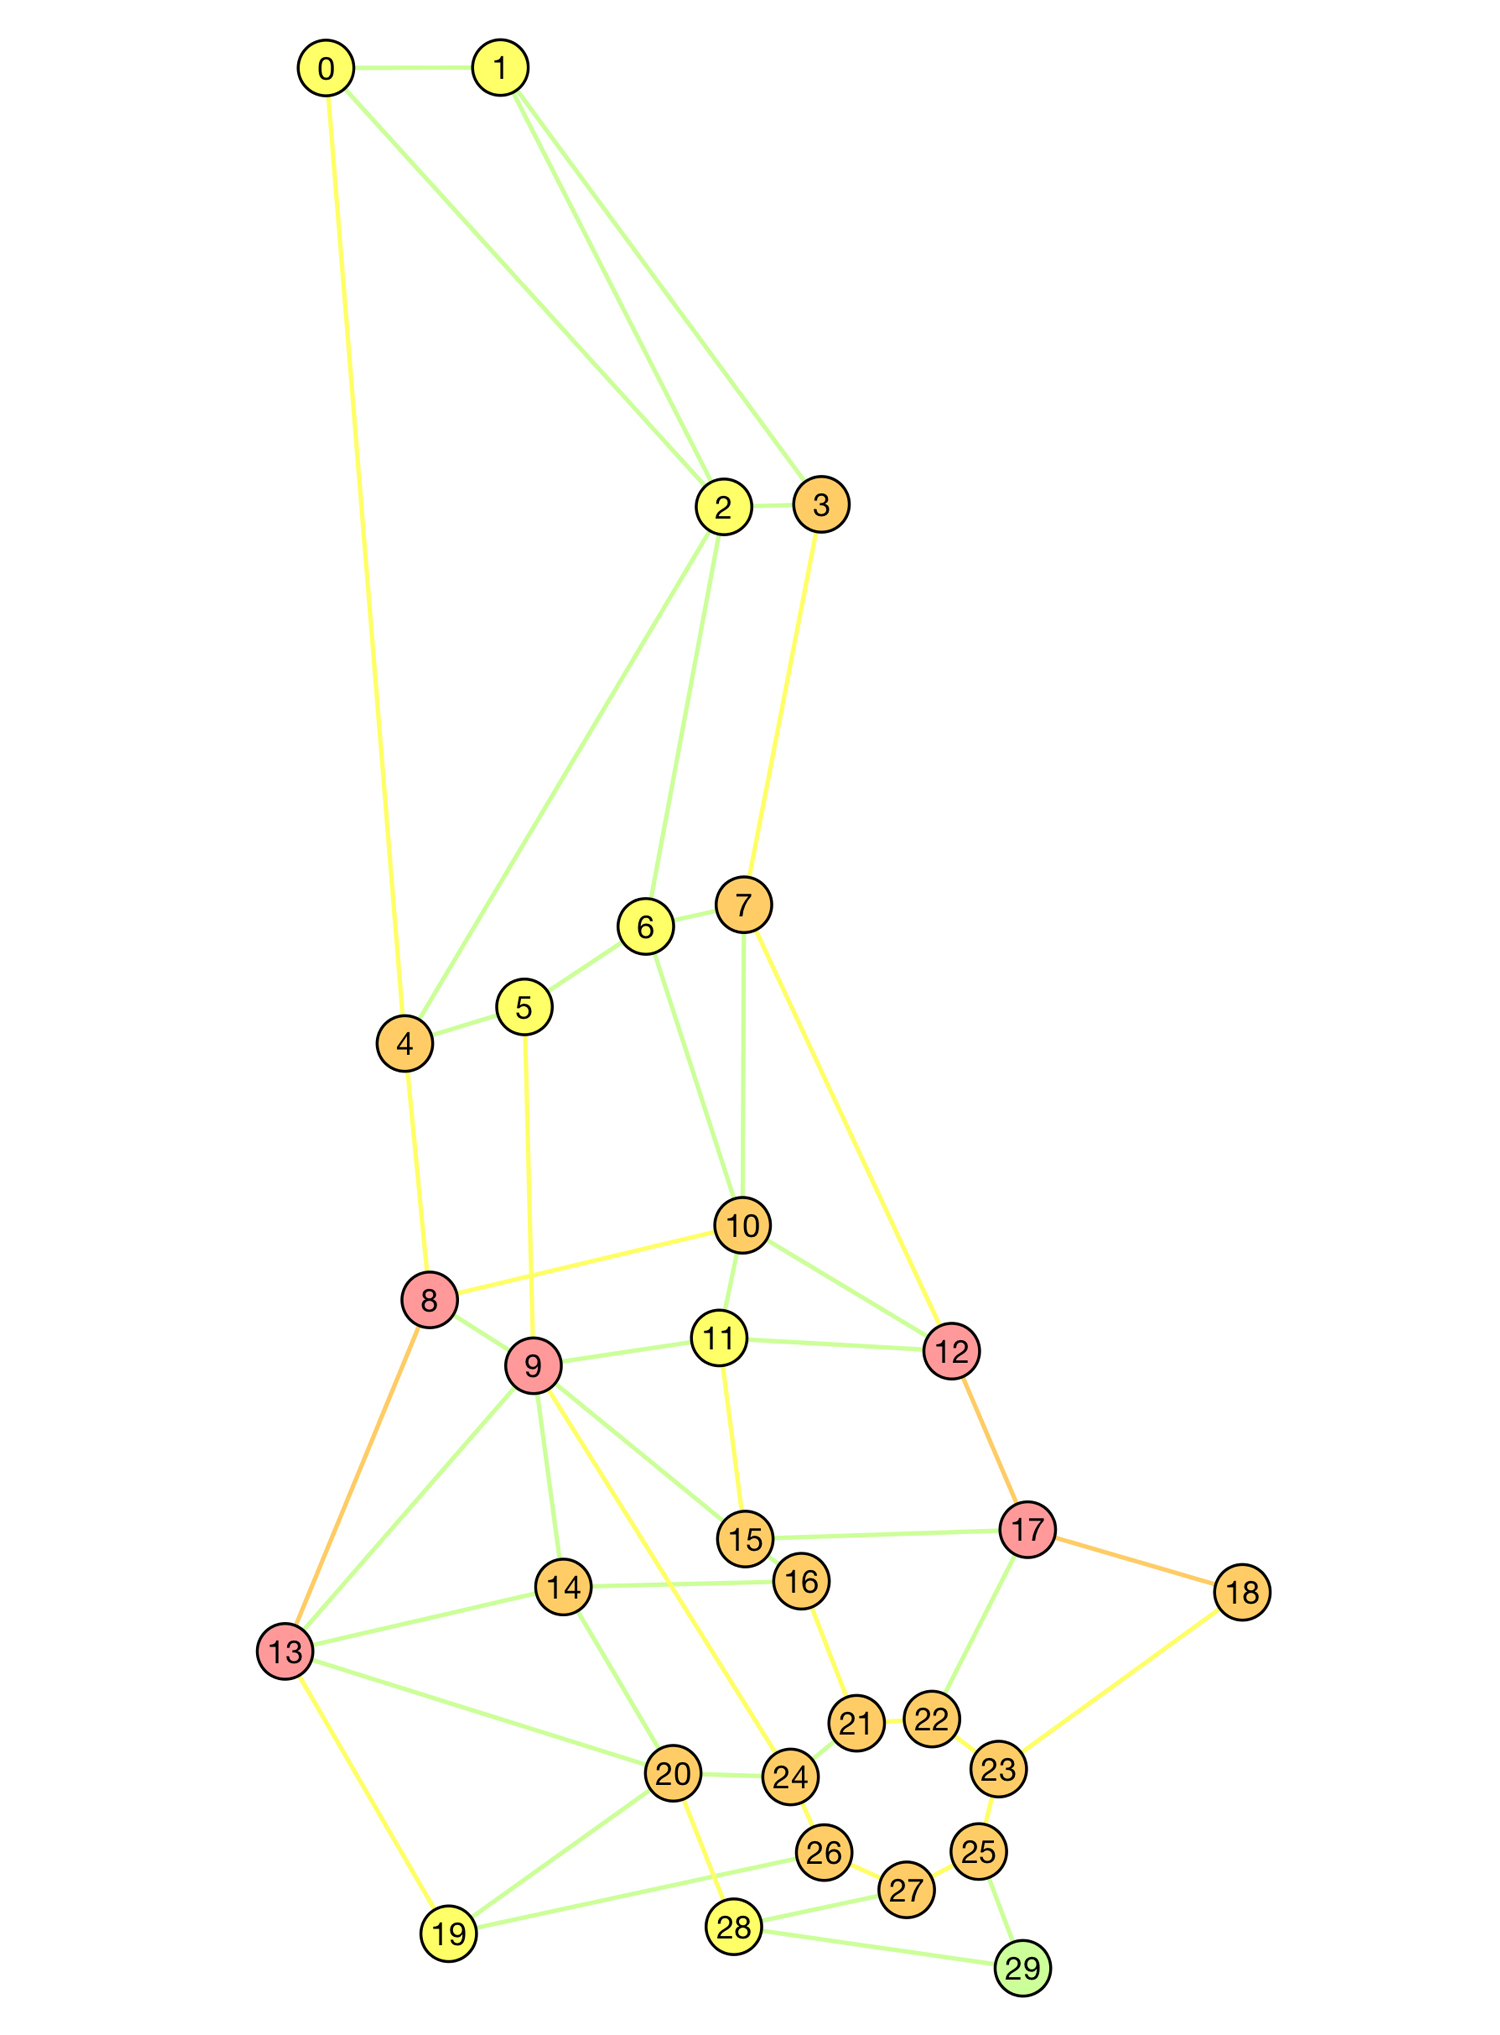
\includegraphics[width=0.47\textwidth]{figs/btc.jpg}
  \caption{A representation of the network being run by the ant-based algorithm at time $t = 10,000$.}
  \label{fig:btc}

\end{figure}

-The length of a run is 500 time steps for initialization (where no load is on the network) followed by 15,000 time steps with load for simulation.

\section{Results}
\label{sec:results}

The main metric used to measure the effectiveness of the ant-based algorithm was the number of calls dropped over the 15,000 time step simulation. We compared our algorithm to breadth-first search as a naiive shortest-path, non-adaptive algorithm, as well as Dijkstra's Algorithm, a least-weight algorithm which we modified to use node weights instead of edge weights.\\

\begin{figure}[htb]
  \centering
  \begin{tabular}{|c|c|c|} 
     \hline % draws two horizontal lines at the top of the table
     & Mean & SD \\ 
    \hline % line after the column headers
    Breadth-First Search & $11.99\%$ & $0.33\%$ \\
    Ant-Based ($0\%$ Noise) & $4.87\%$ & $0.35\%$\\
    Ant-Based ($5\%$ Noise) & $5.24\%$ & $0.40\%$\\
    Dijkstra's Algorithm & $0.11\%$ & $0.04\%$\\
    \hline
  \end{tabular}
  \caption{Percentages of dropped calls over 10 runs of 15,000 time steps.}
  \label{tab:results}

\end{figure}

The call dropping seemed to cycle slightly, as the network became more and less congested. Additionally, with the ant-based algorithm, results seemed to get slightly worse over time, though not severely. 

\begin{figure}[htb]

  \centering
  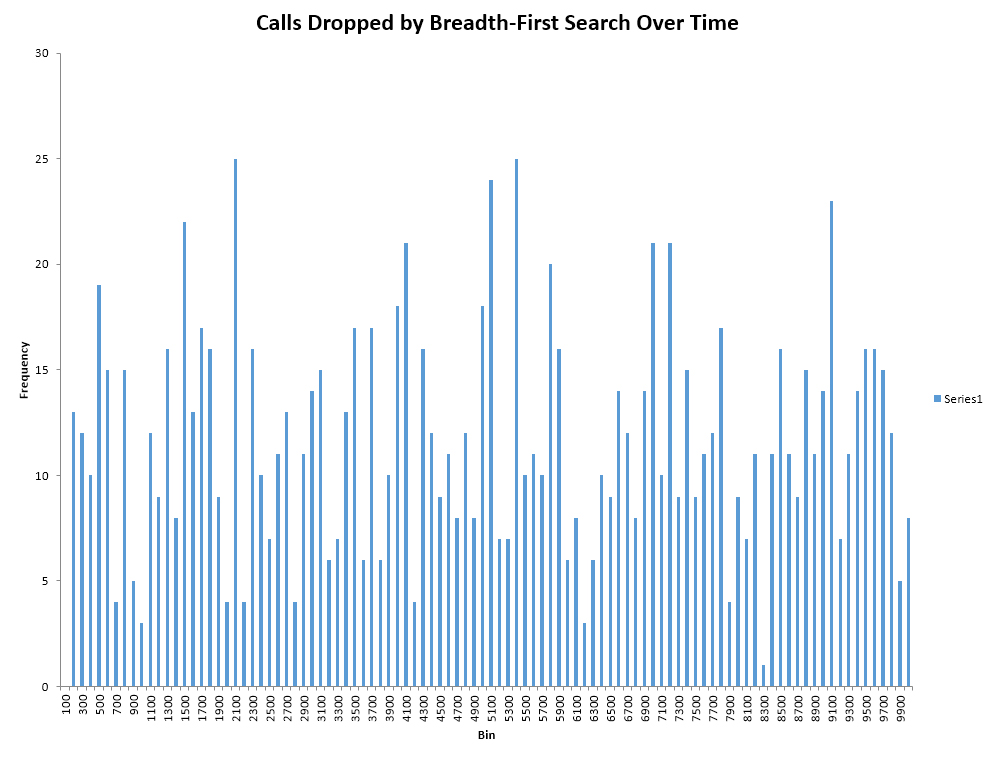
\includegraphics[width=0.47\textwidth]{figs/bfs_hist.jpg}
  \caption{Calls dropped by breadth-first search.}
  \label{fig:bfs_hist}

\end{figure}

\begin{figure}[!h]

  \centering
  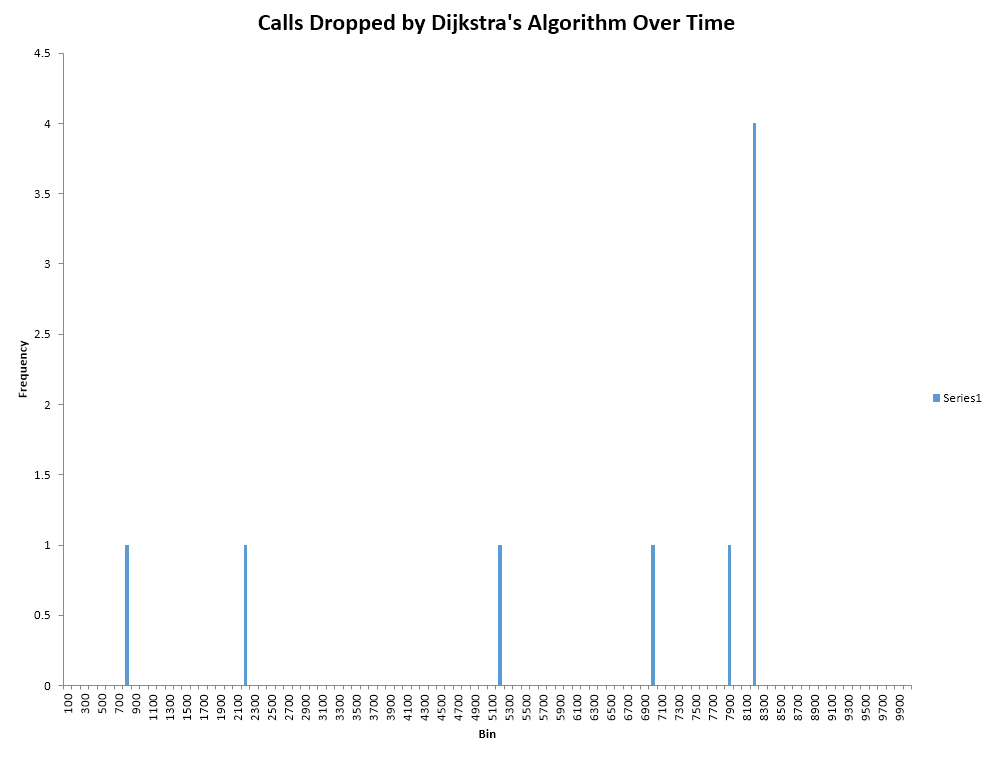
\includegraphics[width=0.47\textwidth]{figs/dijk_hist.jpg}
  \caption{Calls dropped by Dijkstra's algorithm.}
  \label{fig:dijk_hist}

\end{figure}

\begin{figure}[htb]

  \centering
  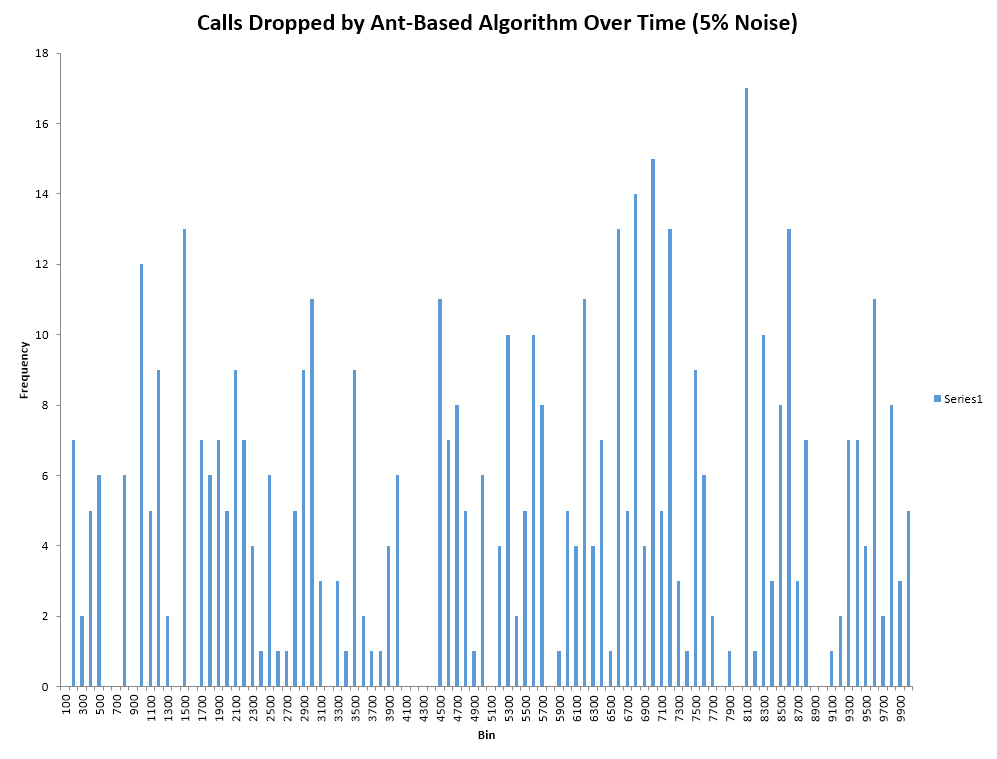
\includegraphics[width=0.47\textwidth]{figs/ant_hist.jpg}
  \caption{Calls dropped by the ant-based algorithm.}
  \label{fig:ant_hist}

\end{figure}

The ant population in this model rose quickly but ended up converging to around 3500 ants. When tested with 100\% noise, the ant population continuously kept climbing, creating an unnecessary processing strain. This is the primary advantage of having ants follow the pheromone trails, it seems; it keeps the ant population at a managable size.

\begin{figure}[htb]

  \centering
  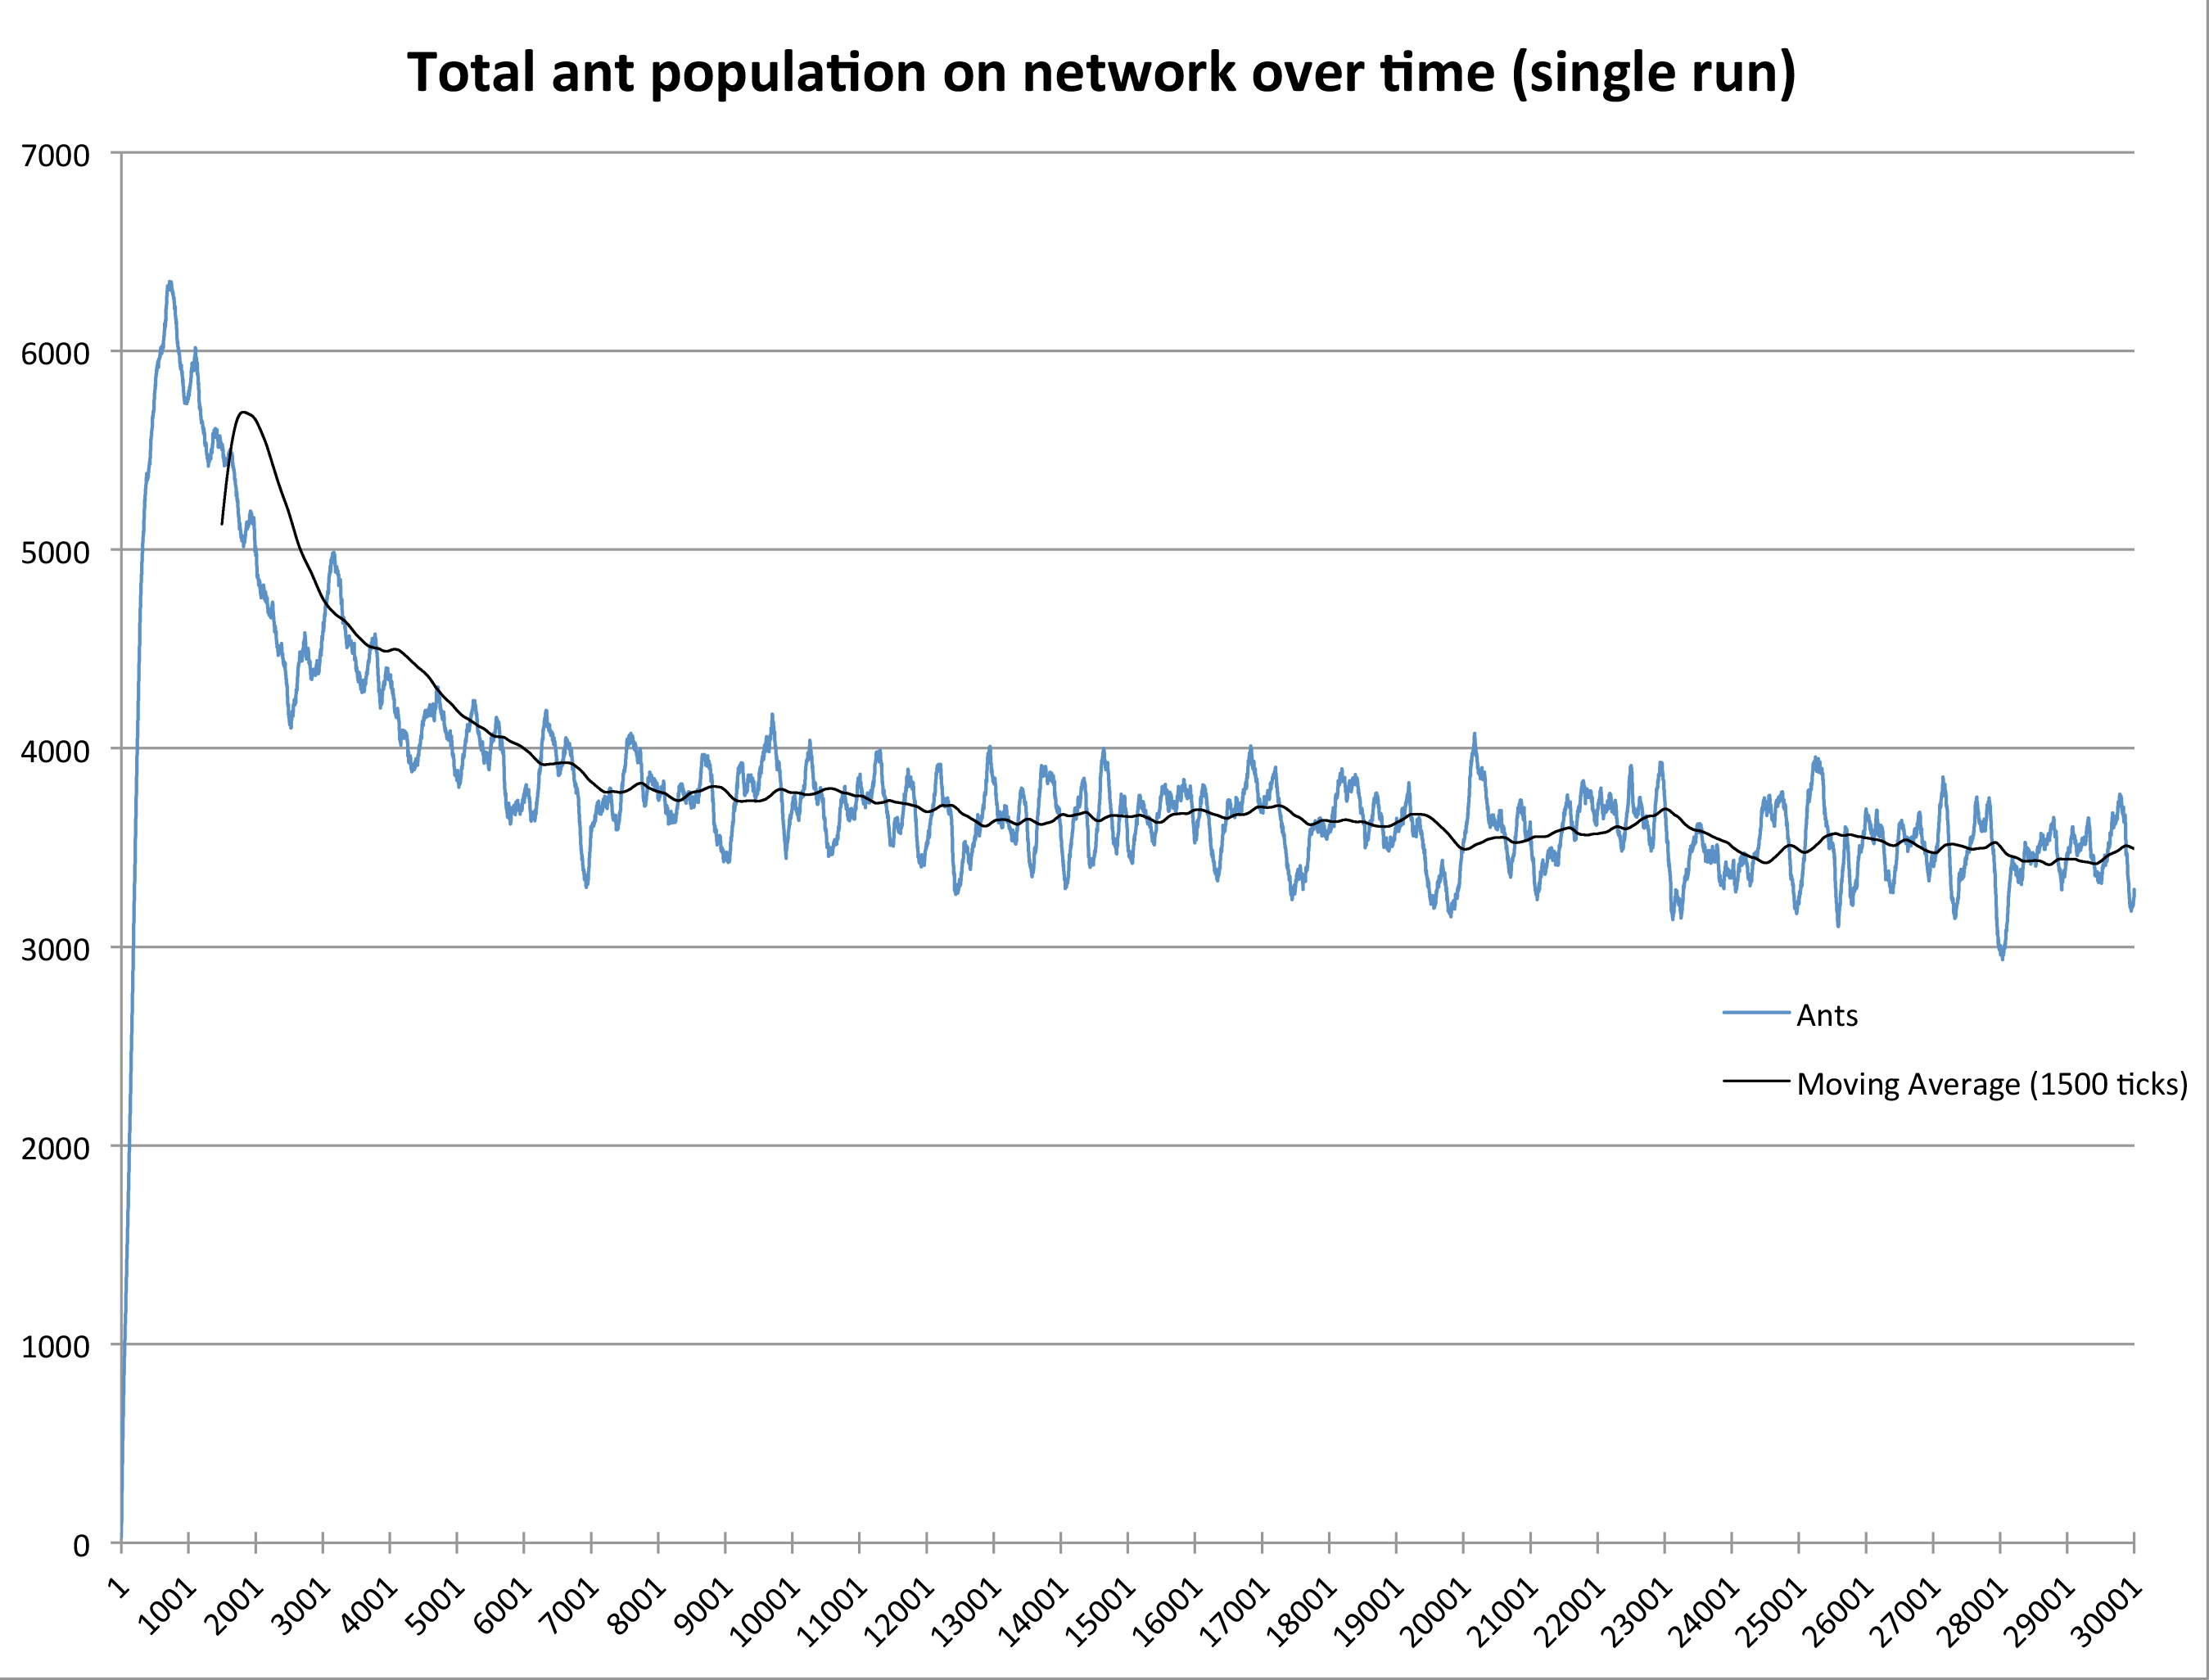
\includegraphics[width=0.47\textwidth]{figs/ant_pop.jpg}
  \caption{Ant population over time.}
  \label{fig:btc}

\end{figure}

\section{Conclusions}
\label{sec:concl}

The ant-based algorithm performs much better than breadth-first search, but does not perform as well as in the results found by Schoonderwoerd et al. However, Dijkstra’s Algorithm outperforms both our implementation of the ant-based algorithm (by nearly a factor of 50) as well as that implemented by Schooderwoerd et al. (by close to a factor of 20). Because of this, Dijkstra’s Algorithm seems to be the best choice to load balance networks (ignoring considerations of time complexity).\\

There are three extensions to this algorithm we would like to explore in the future. First, we would like to test this algorithm on other network topologies. Secondly, implementing a call frequency table to allow specific source nodes to call certain destination nodes more often than others would render a more realistic simulation of how calls are generally placed. Finally, we think it would be interesting to try the same experiment with non-uniform maximum node capacities.

\section{Acknowledgements} 
\label{sec:ack} 

Thanks to Dr. Raghu Ramanujan for his support throughout this project!
\section*{References}
\label{sec:bib}

Schoonderwoerd, Ruud, Owen Holland, Janet Bruten, and Leon Rothkrantz. 1996. "Ant-based load balancing in telecommunications networks." Adaptive Behavior 169-207.\\

\noindent "BT 21CN - Network Topology \& Technology." Kitz - ADSL Broadband Information Site. 29 Apr. 2015.

\end{document}
